\documentclass{beamer}

% Preamble
\usepackage[latin1]{inputenc}
\usetheme{Warsaw}

% Title page
\title[Git - Version Control System]{Introduction  to Version Control with Git}
\author{Andreas Skielboe}
\institute{Dark Cosmology Centre \\ Niels Bohr Institute}
\date{\today}

% Settings
\def \figureHeight {130px}

\begin{document}

\begin{frame}
	\titlepage
\end{frame}

\begin{frame}{License}
	All images adapted from {\bf Pro Git} by Scott Chacon and released under license Creative Commons BY-NC-SA 3.0.
\end{frame}

\begin{frame}{Why Use Version Control?}
	A Version Control System (VCS) is an integrated fool-proof framework for
	\begin{itemize}
		\item Backup and Restore
		\item Short and long-term undo
		\item Tracking changes
		\item Synchronization
		\item Collaborating
		\item Sandboxing
	\end{itemize}
	... with minimal overhead.
\end{frame}

\begin{frame}{Local Version Control Systems}
	Conventional version control systems provides some of these features by making a local database with all changes made to files.
	\begin{figure}
		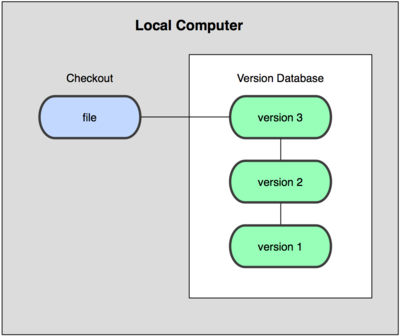
\includegraphics[height=\figureHeight]{images/local-version-control.png}
	\end{figure}
	Any file can be recreated by getting changes from the database and patch them up.
\end{frame}

\begin{frame}{Centralized Version Control Systems}
	To enable synchronization and collaborative features the database is stored on a central VCS server, where everyone works in the same database.
	\begin{figure}
		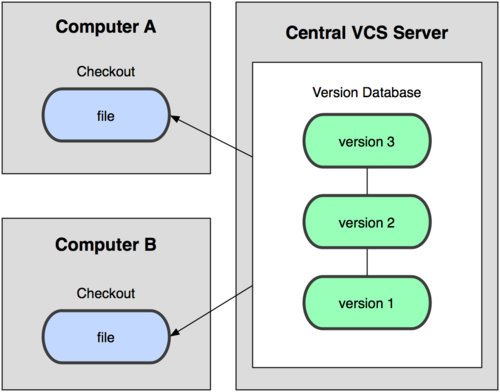
\includegraphics[height=\figureHeight]{images/central-version-control.png}
	\end{figure}
	Introduces problems: single point of failure, inability to work offline.
\end{frame}

\begin{frame}{Distributed Version Control Systems}
	To overcome problems related to centralization, distributed VCSs (DVCSs) were invented. Keeping a complete copy of database in every working directory.
	\begin{figure}
		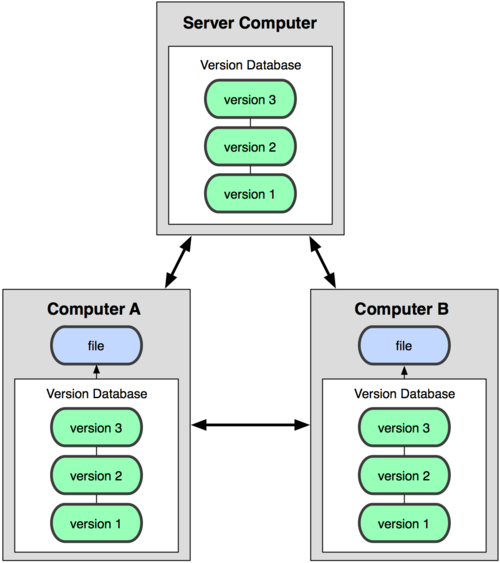
\includegraphics[height=\figureHeight]{images/distributed-version-control.png}
	\end{figure}
	Actually the most {\bf simple} and most {\bf powerful} implementation of any VCS.
\end{frame}

% % % Git Basics % % %
\begin{frame}{Git Basics}
	\begin{center}
		Git Basics
	\end{center}
\end{frame}

\begin{frame}{Git Basics - The Git Workflow}
	The simplest use of Git:
	\begin{itemize}
		\item {\bf Modify} files in your \emph{working directory}.
		\item {\bf Stage} the files, adding snapshots of them to your \emph{staging area}.
		\item {\bf Commit}, takes files in the staging area and stores that snapshot permanently to your \emph{Git directory}.
	\end{itemize}
\end{frame}

\begin{frame}{Git Basics - The Three States}
The three basic states of files in your Git repository:
\begin{figure}
   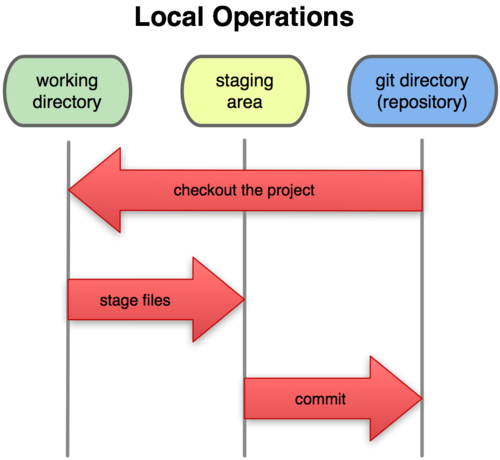
\includegraphics[height=\figureHeight]{images/the-three-states.png}
\end{figure}
\end{frame}

\begin{frame}{Git Basics}
Basic characteristics of Git:
\begin{itemize}
  \item Nearly every operation is local (speed, availability)
  \item Committed snapshots are always kept (integrity)
  \item Strong support for non-linear development (branching, merging, experimentation)
\end{itemize}
\end{frame}

\begin{frame}{Hands-on}
	\begin{center}
		Hands-on with Git
	\end{center}
\end{frame}

\begin{frame}[fragile]{First-Time Git Setup}
	Before using Git for the first time:
	\begin{exampleblock}{Pick your identity}
		\begin{verbatim}
			$ git config --global user.name "John Doe"
			$ git config --global user.email johndoe@example.com
		\end{verbatim}
	\end{exampleblock}
	
	\begin{exampleblock}{Check your settings}
		\begin{verbatim}
			$ git config --list
		\end{verbatim}
	\end{exampleblock}
	
	\begin{exampleblock}{Get help}
		\begin{verbatim}
			$ git help <verb>
		\end{verbatim}
	\end{exampleblock}
\end{frame}

\end{document}